\documentclass[sigconf]{acmart}

\usepackage{booktabs} % For formal tables


% Copyright
%\setcopyright{none}
%\setcopyright{acmcopyright}
%\setcopyright{acmlicensed}
%\setcopyright{rightsretained}
%\setcopyright{usgov}
%\setcopyright{usgovmixed}
%\setcopyright{cagov}
%\setcopyright{cagovmixed}


% DOI
%\acmDOI{10.475/123_4}

% ISBN
%\acmISBN{123-4567-24-567/08/06}

%Conference
%MAYBE set this
%\acmConference[WOODSTOCK'97]{ACM Woodstock conference}{July 1997}{El
%  Paso, Texas USA}
%\acmYear{1997}
%\copyrightyear{2016}


%\acmArticle{4}
%\acmPrice{15.00}

% These commands are optional
%\acmBooktitle{Transactions of the ACM Woodstock conference}
%\editor{Jennifer B. Sartor}
%\editor{Theo D'Hondt}
%\editor{Wolfgang De Meuter}


\begin{document}
\title{Linux-Integrated TCP Acceleration as a Service}
%\titlenote{Produces the permission block, and
%  copyright information}
%\subtitle{Extended Abstract}
%\subtitlenote{The full version of the author's guide is available as
%  \texttt{acmart.pdf} document}

\author{Amanda Austin}
\affiliation{
  \institution{University of Texas at Austin}
}
%\email{jsmith@affiliation.org}

\author{Henrique Fingler}
%\authornote{Dr.~Trovato insisted his name be first.}
%\orcid{1234-5678-9012}
\affiliation{
  \institution{University of Texas at Austin}
}
%\email{trovato@corporation.com}


\author{Timothy Stamler}
\affiliation{
  \institution{University of Texas at Austin}
}
%\email{jsmith@affiliation.org}

% The default list of authors is too long for headers.
%\renewcommand{\shortauthors}{B. Trovato et al.}


\begin{abstract}
Netowkring speeds have increased while CPU speeds have not. As a result, an
increasing portion of packet processing time is spent in the kernel
networking stack. To mitigate this effect, TCP Acceleration as a Service
(TAS) splits TCP processing into a fast path and a slow path, both of which
operate as userspace processes. In doing so, however, TAS loses some
information about the network when compared to an in-kernel networking stack
(e.g., firewalls, ARP tables). We present a Linux-integrated TAS that
interfaces with Linux via a virtual network device. TAS duplicates some slow
path packets to Linux via this virtual device, observes Linux's response,
and then mimics that response. We show that this method can allow TAS to use
Linux's information about the network while retaining the performance of TAS
fast path operations.
\end{abstract}

%
% The code below should be generated by the tool at
% http://dl.acm.org/ccs.cfm
% Please copy and paste the code instead of the example below.
%
%\begin{CCSXML}
%<ccs2012>
% <concept>
%  <concept_id>10010520.10010553.10010562</concept_id>
%  <concept_desc>Computer systems organization~Embedded systems</concept_desc>
%  <concept_significance>500</concept_significance>
% </concept>
%</ccs2012>
%\end{CCSXML}

%\ccsdesc[500]{Computer systems organization~Embedded systems}
%\ccsdesc[300]{Computer systems organization~Redundancy}
%\ccsdesc{Computer systems organization~Robotics}
%\ccsdesc[100]{Networks~Network reliability}


%\keywords{ACM proceedings, \LaTeX, text tagging}

\maketitle


\section{Introduction}\label{Introduction}

Networking speeds have become faster while CPUs have not, causing network packet
processing efficiency to become important for datacenter networks. Datacenter
applications continue to want high throughput and low latency access to the
network along with the guarantees provided by TCP: lossless in-order delivery of
packets, but this comes at the cost of consuming an increasing fraction of CPU
processing resources. For example, nearly 70\% of packet processing time for a
simple echo server application is spent in the Linux networking stack 
\cite{peter:arrakis}.

To cope with this, many alternative TCP stacks have been proposed that seek to
increase the efficiency of packet processing. TAS (TCP Acceleration as a
Service) splits TCP packet processing into a fast path and a slow path. The fast
path handles common data path operations such as handling in-order delivery of
packets from established connections and generating acknowledgements. The slow
path handles less common, control path operations such as connection management,
congestion control, and connection timeouts. Both the fast path and slow path
operate as user-level processes.

Implementing a TCP stack in userspace comes with a few drawbacks. Namely, the
Linux TCP stack contains a lot of functionality and information about the
network that is hard to replicate in userspace. Ideally, a userspace networking 
stack should make the same decisions about connection management, security,
congestion, etc. as the Linux stack.

We present Linux-Integrated TCP Acceleration as a Service, an extension to TAS
that interfaces with Linux for some slow path operations. The slow path now
sends some packets to Linux, observes Linux's response, and mimics it. In this
way, TAS can gain some of the information and functionality of the Linux TCP
stack, such as firewall and network information (e.g., ARP tables), while
retaining the performance of fast path operations.

Our paper makes the following contributions:

\begin{itemize}
\item We design and implement a method for the TAS to interface with Linux for
  some slow path operations (connection setup and teardown, ARP) in order to
  gain information and functionality.

\item We evaluate our implementation and show that we introduce no overheads
  for fast path operations. Connection setup and ARP slow down significantly,
  but these operations are uncommon enough that they do not affect the
  throughput seen by the application.
\end{itemize}

In the remainder of our paper, we provide some background on TAS and virtual
network devices in Section \ref{Background}. We discuss the design and
implementation of Linux-integrated TAS in Section \ref{Design}. We evaluate
our implementation in Section \ref{Eval} and finally conclude and discuss
future work in Section \ref{Conclusion}.

\section{Background}\label{Background}


* TCP stack types
** kernel
** user level
** hybrid
** other (offload, dedicated cpu)

*split tcp

\begin{figure}
\centering
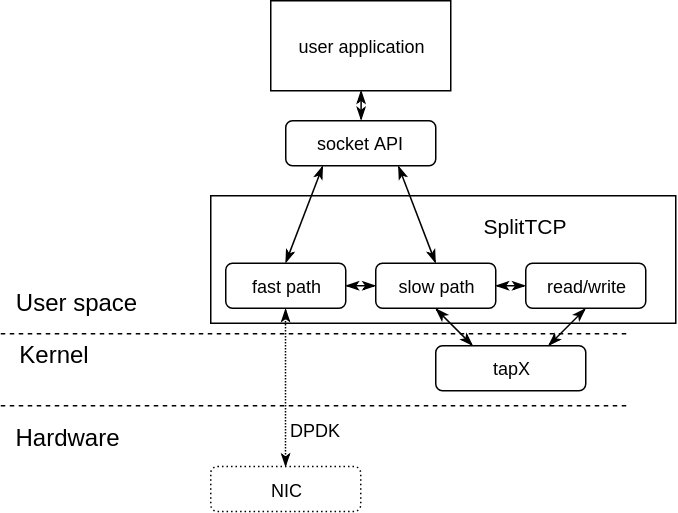
\includegraphics[width=\columnwidth]{figures/splittcp.png}
\caption{TBD.}
\label{fig:splittcp}
\end{figure}


* functionality glue

* Tap devices


\begin{figure}
\centering
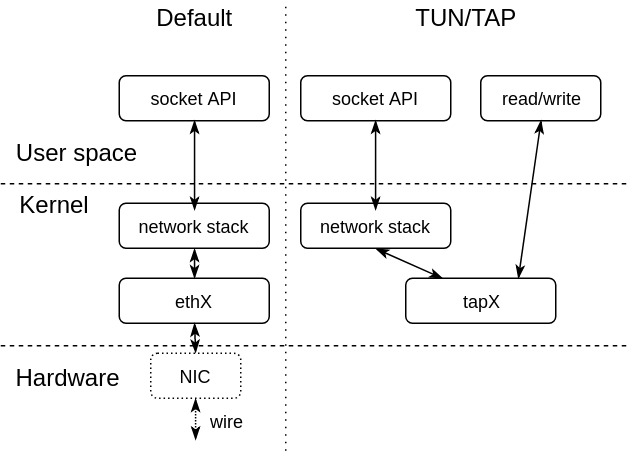
\includegraphics[width=\columnwidth]{figures/tap_diag.png}
\caption{TBD.}
\label{fig:tap}
\end{figure}

\section{Design}\label{Design}

\subsection{TAS Design}

TAS seeks to address a number of problems in the realm of datacenter packet
processing such as efficiency, predictability, and workload proportionality. 
Several important design decisions were made to accomplish these, but we will 
focus on just two of those: the split into a fast path and a slow path, and the
implementation of a userspace TCP stack.

One key way that TAS achieves high connection scalability and 
predictability is by dividing TCP functionality into two components: a fast 
path and a slow path. The fast path handles common-case packets and detects 
exceptions that need to be handled in the slow path. The main functions that
the fast path handles are common case send/receive, where the fast path directly
reads or writes packet payloads from application buffers and interacts directly
with the network, fast ACK handling, where the fast path will either generate or
consume ACK packets quickly without having to invoke the slow path, and 
efficient exception recognition and forwarding. 

In doing this, heavyweight TCP operations are taken out of the data path and 
relegated to the slow path, where they can be handled without affecting the 
performance of other flows in the fast path. The slow path does costly, 
infrequent operations like connection setup and teardown, timeouts, and 
enforcing congestion control. The slow path also handles out of order packets, 
but these are very infrequent in a datacenter environment.
   
In order for this separation and the individual components of the fast path 
and slow path to stay efficient, everything is implemented in a userspace TCP
stack. This provides all the normal functionality of TCP without having to 
switch back and forth between user and kernel space. This is good for 
performance and ease of programming, but isolates the TCP stack from Linux.
While we don't want to rely on Linux for performance operations, it does contain
information about the network and a configurability that would be useful in a 
datacenter environment.

\subsection{Integration Goals}

To most effectively interface with Linux, we take advantage of the previously 
described TAS design choices in order to minimize our impact on common case
packet processing. 

First, we don't make any modifications to the fast path code or data structures.
We prioritize making changes around the fast path, but add no additional lines 
of code to common case packet processing, and no additions and minimal 
interaction with fast path data structures to avoid incurring contention, cache 
problems, or race conditions. By following this rule, we shouldn't incur any
direct overheads to the cases that we care most about.

Secondly, we don't worry about performance in the slow path as long as it
doesn't incur any scheduling or blocking problems with the fast path. We have 
very little control over how often Linux will deliver packets to the slow path, 
so we want to make sure this doesn't negatively affect the fast path threads 
when they might be co-scheduled with the slow path.

\subsection{Compromises Made}

In order to accomplish these goals, we made some compromises to certain problems
in our implementation. In these cases, we could have used few lines of code or 
perhaps gotten better performance for the slow path operation, but at the 
expense of potentially slowing down the fast path.

First, as previously discussed, the fast path naturally consumes all ACK packet,
including during connection setup. In order to most faithfully setup the 
connection, we would need to modify the fast path to either forward ACK packets 
to the slow path, or write packets directly to the tap device. Instead of 
absorbing these costs in the fast path, we instead manually create a new ACK
packet during connection setup in the slow path and write it to the tap device.

Second, we maintain separate sequence numbers between Linux and TAS and 
between TAS and remote hosts. TAS immediately initializes fast path 
state upon receiving a \textit{SYN} packet and doesn't update it after that unless 
there's some kind of exception. Although this takes place in the slow path,
this would require adding some kind of complexity, as we won't know the sequence
number Linux wants to use until it provides a \textit{SYN/ACK}. We can address this by 
doing one of the following: adding an artificial delay or some kind of signal 
from the thread interacting with Linux in the middle of \textit{SYN} processing to make 
sure the sequence number is available when fast path state is initialized, 
initializing fast path state at a later time, modifying the fast path to 
identify either outgoing \textit{SYN/ACK} packets or incorrect outgoing sequence numbers
and adapting, or keeping separate sequence numbers. The final solution ended up 
being the simplest; the first will slow down connection setup even more, the 
second may create additional race conditions or problems in connection setup, 
and the last will slow down the fast path in some way.

Third, similarly to the first compromise, we handle ARP packets manually in 
the slow path, as they are not always forwarded to the slow path. By default,
the fast path only forwards ARP packets to the slow path if it is an IP address
that it doesn't have state for. As connection state is initialized immediately 
upon a \textit{SYN} packet being received, if we try to forward any Linux ARPs to the 
network for that connection, the replies will be dropped by the fast path. In
this case, instead of forwarding all ARP packets to the slow path or delaying
initializing connection state again, we fake ARP responses to Linux requests 
in the slow path by searching TAS's ARP table and manually crafting 
packets. 

\begin{figure}
\centering
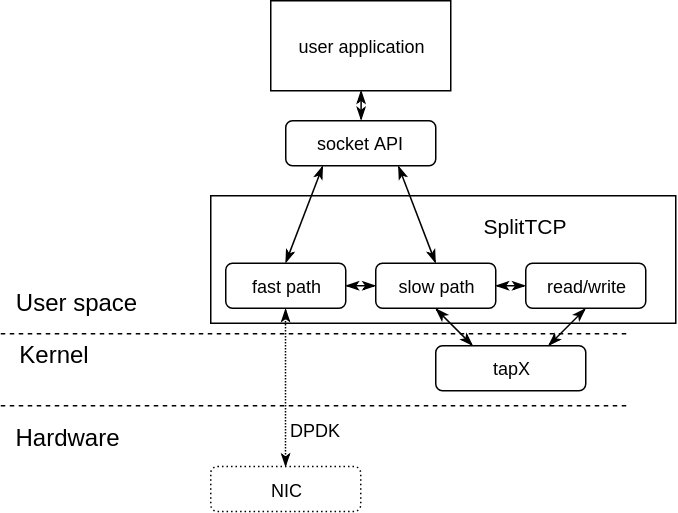
\includegraphics[width=0.7\columnwidth]{figures/splittcp.png}
\caption{Design of TAS with kernel integration. TAS now replicates all slow path operations to the kernel, checks what
it did by reading raw packets from the TAP device and mimics its decisions.}
\label{fig:splittcp_tap}
\end{figure}


%\section{Implementation}

In order to achieve a Linux-integrated SplitTCP implementation, the following 
changes were implemented and functionalities added.

\subsection{Tap Initialization and Interaction}

At the time of SplitTCP's initialization, a tap device is created with Linux.
We control the name and IP of this tap device, but Linux and anyone using the
operating system with root privileges can configure it to do whatever they
want, and SplitTCP will reflect these changes. At initialization, we need to
save the MAC address that is assigned to the tap device so that future packets
written to the tap device can copy and use it. 

Writing packets to the tap device is simple and can be done from anywhere in the
slow path. It is merely a function call with the buffer and a length, but we 
make sure to copy the saved MAC address for the tap device over the desination
MAC field in any packets being written to the tap device. 

Reading packets from the tap device is done in a separate thread that can block
with epoll while waiting for packets to be received from Linux. Once packets are
received, they are parsed and handled according to headers, flags, and existing
connection state. With this parsing already done, it enables us to more easily
handle more types of Linux packets and add more functionality. 

\subsection{Tap Control Packets and Network Interface}

To more easily create and format packets to write to the tap device, a new
interface was written based on the existing SplitTCP control packet creation
interface, but reversed. When a control packet such as an ACK needs to be 
generated, connection state is looked up and crafted into a packet, with
SplitTCP being the source and the remote host being the destination. Instead,
with our tap control interface, a packet is crafted with the remote host as
the source and Linux as the destination. This reversal applies to IP addresses,
MAC addresses, sequence and acknoledgement numbers, and TCP timestamp options.

In addition to a new interface for generating packets for the tap device, a new
interface was needed for forwarding raw packets from the tap device to the 
network. By default, SplitTCP only has the existing control interface for 
creating and sending certain packets to the network from the slow path, but 
not an interface for sending raw buffers directly to the network. We added this
functionality so that we can forward packets directly from Linux to the remote
host with minimal modifications.

\subsection{Modified Socket Library}

Because Linux does not just acknowledge arbitrary SYN packets, we had to do some
extra work at the library level in order to prepare Linux. Typically, the 
application would interact with Linux through the socket library, but with 
SplitTCP, all socket operations are intercepted and forwarded instead of being
delivered to Linux. In this environment, Linux is completely unaware of the 
application listening for connections. To rectify this, we duplicate all 
necessary socket operations through libc. When the application calls a socket 
operation that we need, the interposition layer on top of libc will call both 
SplitTCP and libc so that Linux is aware of all the same information that 
SplitTCP is. The functions we currently handle for this are socket, bind, 
fcntl, setsockopt, listen, and accept. 

To make sure that file descriptors aren't getting mixed up, we maintain a map
of SplitTCP file descriptors to Linux file descriptors and only return SplitTCP
descriptors to the application. Whenever one of the aforementioned functions is 
called, the SplitTCP file descriptor provided by the application is 
cross-referenced with the map in order to find the proper file descriptor to use
with libc. 

\subsection{ARP Support}

In our implementation of SplitTCP, Linux cannot interact directly with remote 
hosts, and ARP requests and replies are no longer handled after connection state
is initialized. Because Linux will likely need to do an ARP request to obtain 
the remote host's MAC address, and because we don't want to make any 
modifications to the fast path, we handle ARP requests in the slow path.

ARP replies are generally sent by the host to which the corresponding address
belongs, but in order to provide Linux the information it needs we fake these 
replies inside the slow path. Upon receiving an ARP request from Linux, we 
search through SplitTCP's ARP table to see if the address is there. If it is, 
we generate a reply and write it back to Linux. If it is not, we forward the 
packet to the network. Because SplitTCP was unaware of this address, we know
it does not maintain any connection state for it, and the corresponding ARP 
reply should be forwarded to the slow path, where it can be written to the tap
device. 

\subsection{Connection Setup}

Finally, we will outline the general changes we had to make to SplitTCP to get
it to cooperate with Linux during connection setup. Once the SYN packet arrives,
 it will naturally be forwarded to the slow path for
connection establishment. After allowing SplitTCP to do its normal connection 
state initialization, we write the SYN packet to Linux. At this point, SplitTCP
would generate an event for the SYNACK to be generated asynchronously. We remove
this funcationality and instead wait for Linux to send a SYNACK. Linux will 
first do an ARP request, which we handle, followed by a SYNACK. We forward this
SYNACK to the network, then do the normal SplitTCP work of updating the 
connection state and signalling the application, as well as the additional work 
of generating an ACK packet to send to Linux. 



\section{Evaluation}\label{Eval}

In this section, we evaluate our implementation of Linux-Integrated TAS. Our
evalutation seeks to answer the following questions:

\begin{itemize}
    \item Do our changes affect the performance of the fast path?
    \item What is the performance of the slow path?
\end{itemize}

\subsection{Evaluation Setup}

To answer the above questions, we run a simple RPC echo server microbenchmark. A  
client sends a packet with a 64 byte payload to a server, which echos the packet
back to the client. Both client and server are single threaded. The server 
machine is an Intel Xeon Gold 6138 system at 2.0 GHz with a 1G NIC. The client 
machine is an Intel Xeon E3-1225 v3 system at 3.3 GHz with a 1G NIC. Both client 
and server run Linux kernel 4.18.

\subsection{Fast Path Performance}

\begin{table}[]
\begin{tabular}{@{}crrrrrr@{}}
\toprule
               & \multicolumn{6}{c}{Latency (us)}                                                                                                                                    \\ \midrule
               & \multicolumn{3}{c}{TAS}                                                          & \multicolumn{3}{c}{Linux-Integrated TAS}                                         \\
\# Connections & \multicolumn{1}{c}{Avg} & \multicolumn{1}{c}{99\%} & \multicolumn{1}{c}{99.99\%} & \multicolumn{1}{c}{Avg} & \multicolumn{1}{c}{99\%} & \multicolumn{1}{c}{99.99\%} \\
1              & 60                      & 70                       & 79                          & 61                      & 62                       & 78                          \\
2              & 63                      & 65                       & 97                          & 62                      & 64                       & 82                          \\
4              & 65                      & 68                       & 105                         & 65                      & 89                       & 118                         \\
8              & 71                      & 79                       & 147                         & 70                      & 78                       & 151                         \\
16             & 68                      & 77                       & 144                         & 69                      & 76                       & 146                         \\
32             & 72                      & 97                       & 170                         & 74                      & 104                      & 153                         \\ \bottomrule
\end{tabular}
\label{fastpath-latency}
\end{table}

Table \ref{fastpath-latency} shows the average and tail latencies of the RPC 
echo microbenchmark with TAS and Linux-Integrated TAS. The average-case latency
of the fast path of Linux-Integrated TAS is within 3\% of TAS. The performance 
at the tail varies a bit more between the two versions, but is within 25\% of 
TAS in the worst case.

Figure \ref{fig:fastpath-throughput} shows the throughput of the RPC echo server
microbenchmark using the original TAS and Linux-Integrated TAS. The throughput 
of both versions are very similar.

\paragraph{Discussion.} Our evaluation results show that the fast path 
performance of Linux-Integrated TAS is very similar to the fast path performance 
of the original TAS. This result aligns with the fact that we made no changes to
the fast path. Additionally, slow path operations such as connection setup and
teardown happen infrequently enough that they do not affect the performance of 
the fast path.

\begin{figure}
  \centering
  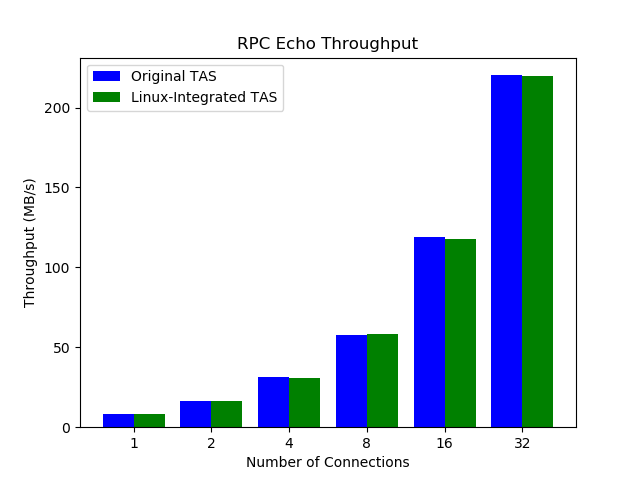
\includegraphics[width=\columnwidth]{figures/rpc_echo_throughput.png}
  \caption{RPC echo throughput for a single threaded client and server.}
  \label{fig:fastpath-throughput}
\end{figure}

\subsection{Slow Path Performance}

Our performance results show that the slow path performance is reduced 
drastically compared to the original TAS. Connection setup times were reported 
on the order of seconds. This is due to the fact that we now incur system call 
overheads on the slow path. We must wait for Linux to handle the packets we send 
to it before we can observe its response. For example, we must issue a blocking 
accept call to Linux to ensure that TAS does not prematurely move on to the next 
connection before observing Linux's response.

\section{Conclusion}\label{Conclusion}

%*No loss of performance on fast path

Integrating kernel functionality into TAS did not affect the fast path operations, which is where
it gets most of its performance benefits.
%*Slow path is hit, but is not frequent
The slow path took a hit in performance due to proxying system calls on every slow path
operation and having to read/write from a TAP device, which incurs plenty of mode switches.
%*Goal was to add functionality, not increase performance
Because slow path operations are infrequent, we think that the tradeoff of slower connection setup
and teardown is worth it to add powerful kernel network functionality such as packet filtering without
having to reimplement it all in user space.




\bibliographystyle{ACM-Reference-Format}
\bibliography{paper}

\end{document}
